\subsection{Particle dynamics}\label{sec:particle_dynamics}

The curvature of the Parker spiral is small over a length scale of
$\sim100\,000\,$\si{km}, which we will later confirmed through comparison with
the particle motion. We can therefore assume the background field is uniform
$\vb{B}_0=B_0\zhat$. Given a vector potential $\vb{A}=\vb{A}_w+xB_0\yhat$ and a scalar potential $\Phi_w$ where $\vb{A}_w,\Phi_w$ are defined as in \cref{sec:whistler}, the relativistic Hamiltonian for a particle with mass $m$ and charge $q$, is
 \begin{equation}\label{eq:relativistic_hamiltonian}
    \HH=\sqrt{m^2c^4+\qty(\vb{P}-q\vb{A}_w-qB_0x\yhat)^2c^2}+q\Phi_w
 \end{equation}
 where $\vb{P}=\gamma m\vb{v}+q\vb{A}$ is the canonical momentum conjugate to
 the Cartesian coordinates and $\gamma$ is the Lorentz factor.

 There are two issues. First, note that $\HH$ depends on $x$, so
 $\dot{P_x}=-\partial\HH/\partial x\neq0$ and $P_x$ is not invariant. Secondly,
 $\vb{A}_w$ oscillates with the phase $\psi(x,z,t)$. So the energy is not
 conserved as the Hamiltonian is time-dependent. The former is a standard
 problem since $\HH$ is currently formulated in Cartesian coordinates, whereas
 the system is cylindrically symmetric due to the background magnetic field.
 This can be resolved by transforming into a cylindrical frame
 \citep{Goldstein2002}. The latter is, however, more problematic as the wave
 introduces oscillations symmetric about its direction of propagation. In-depth
 analysis of the Hamiltonian can be done by using secular perturbation theory
 \citep{Lichtenberg&Lieberman1992}, which involves decomposing the Hamiltonian into Bessel-Fourier series and performing the gyro-averaging method to separate a single term, the $n$th harmonic, in the series.


 Within the scope of our analysis, we will calculate this Hamiltonian system's
 adiabatic invariants and derive its resonance surfaces similar to
 the approach of \cite{Karimabadi1990} and \cite{RobergClark2019}.  The mathematical details are given in \cref{sec:hamiltonian_analysis}. For motion near the resonance $n$, the Hamiltonian can be recast into the form
 \begin{equation}\label{eq:1D_hamiltonian}
     \HH(\zeta;\hat{P_\phi},\hat{P_\zeta})
     =\gamma\qty(\hat{P_\phi}+n\hat{P_\zeta},k_\|\hat{P_\zeta})mc^2
     -\omega\hat{P_\zeta}
     +G_n\qty(\hat{P_\phi}+n\hat{P_\zeta},k_\|\hat{P_\zeta})\sin\zeta
 \end{equation}
 where the action-angle variables $(\zeta,\hat{P_\zeta})$ and $(\phi,\hat{P_\phi})$ are
 given by
 \begin{align}
     \zeta&=n\phi+k_\bot P_y/qB_0+k_\| z-\omega t &
     \phi&=\tan^{-1}\qty[\frac{m\Omega_c\qty(x-P_y/qB_0)}{P_x}]\notag\\
     \hat{P_\zeta}&=P_\|/k_\| & \hat{P_\phi}&=P_\phi-nP_\|/k_\|=P_\perp^2/2m\Omega_c-nP_\|/k_\|
 \end{align}
 The perpendicular momentum is defined as
 $P_\perp=\sqrt{P_x^2+\qty(P_y-qB_0x)^2}$. The gyroradius is then
 $\rho=P_\perp/m\Omega_c=\sqrt{2P_\phi}$, and
 the Lorentz factor $\gamma=\sqrt{1+(P_\perp^2/m^2c^2)+(P_\|^2/m^2c^2)}$.
 The perturbation amplitude $G_n$ is defined as
 \begin{equation}
     G_n(P_\phi,P_\|)=mc^2\qty{s\qty[\delta_0+\frac{\delta_1}{\gamma}\qty(\frac{k_\perp}{k}\frac{P_\|}{mc}-\frac{k_\|}{k}\frac{n\Omega_c}{ck_\perp})]J_n\qty(k_\bot\sqrt{2P_\phi})+\frac{\delta_2}{\gamma}\frac{\rho\Omega_c}{c}J_n'\qty(k_\perp\sqrt{2P_\phi})}
 \end{equation}
 where $J_n,J_n'$ are the $n$th order Bessel functions of the first kind and
 their derivatives, the wave potential amplitudes are
 $\delta_0=\abs{q}\Phi_0/mc^2$ and $\delta_{1,2}=\abs{q}A_{1,2}/mc$, and
 $s=q/\abs{q}$ is the charge sign. The equation of motion of this system is
 \begin{subequations}\label{eq:hamiltonian_eom}
    \begin{align}
        \frac{d\zeta}{dt}&=-\omega+\frac{n\Omega_c}{\gamma}+\frac{k_\|P_\|}{\gamma m}+\qty(n\frac{\partial
        G_n}{\partial P_\phi}+k_\|\frac{\partial G_n}{\partial
    P_\|})\sin\zeta\label{eq:dzdt}\\
            \frac{d\hat{P_\zeta}}{dt}&=-G_n\cos\zeta\label{eq:dPdt}
    \end{align}
 \end{subequations}

 \begin{figure}
     \centering
     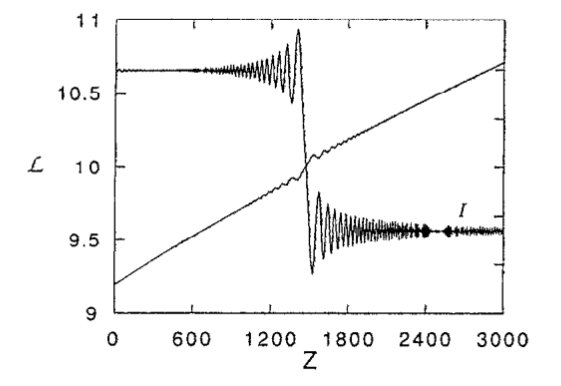
\includegraphics[width=0.6\textwidth]{resonance_crossing.png}
     \caption{The change in the adiabatic invariant $I$ as the resonance
     $\mathcal{L}$ crosses an integer value (figure from \cite{Albert1993}).
 In our notations, $\mathcal{L}=n$, $I=\hat{P_{\phi}}$, and $Z=z$.}
     \label{fig:resonance_crossing}
 \end{figure}
 Here, we have assumed that the wave is small ($\delta_{0,1,2}\ll
 1$ and $\delta_{1,2}<\gamma v/c$, where $v$ is the particle's velocity). So the
 motion $\dot\zeta$ is usually fast, meaning we can average over $\zeta$
 and $\dot{P_\zeta}=0$, except for when
 \begin{equation}\label{eq:resonant_condition}
     \omega=\frac{n\Omega_c}{\gamma}+\frac{k_\|P_\|}{\gamma m}
 \end{equation}
 The adiabatic invariant $\hat{P_\zeta}$ is no longer conserved whenever the particle undergoes a resonance crossing (see \cref{fig:resonance_crossing}). \cref{eq:resonant_condition} then
 describes a resonant condition. Although this is not a convention, most
 literature defines the gyrophase as $s\phi$, which results
 in the resonant mode being $sn$. For an electron with $s=-1$, this means
 their fundamental cyclotron motion is the $n=-1$ mode, while the fundamental
 cyclotron as defined by \cref{eq:resonant_condition} is $n=1$. This definition 
 will be used in subsequent discussions. 

\begin{figure}
     \centering
     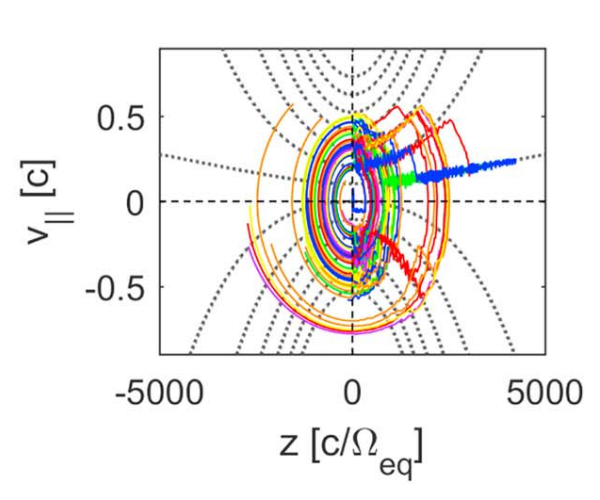
\includegraphics[width=0.6\textwidth]{hsieh_particle_trapped.png}
     \caption{Trajectories (colored solid lines) of particles being trapped
         along (dotted) resonance lines
     ($\abs{n}\leq6$) in \cite{Hsieh2017}.}
     \label{fig:trapped_particles}
 \end{figure}
